\documentclass[10pt,a4paper]{report}
\usepackage{style}
\title{\Huge{\textbf{Le Taquin}}}
\author{Mélanie MARQUES \& Guillaume COQUARD}
\date{Rendu le 18 mars 2019}
\begin{document}
\begin{titlepage}
\maketitle
\end{titlepage}
\chapter{Etude Théorique}
\section{Le Problème du Taquin}
\paragraph{} {Un taquin ${n \times n}$ est un puzzle carré, d'une largeur ${l}$ et d'une taille ${t}$, telles que ${l = n}$, ${t = n \times n}$, composé de ${t - 1}$ tuiles numérotées de 1 à ${t}$ et d’un trou.}
\begin{figure}[!h]
\centering
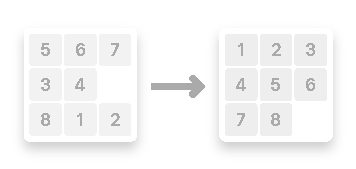
\includegraphics[keepaspectratio=true,width=10cm]{./inc/media/presentation_twoTaquins.pdf}
\end{figure}
\paragraph{} {Les tuiles ne peuvent se déplacer que par glissement dans la seule case vide à un moment donné. Le jeu consiste à replacer les tuiles dans l’ordre numérique. Ainsi, par le biais de ce projet, nous allons donc, à l'aide du langage de programmation {\ttfamily Python}, développer ce jeu et répondre aux deux questions suivantes: Quelle est la séquence minimale de mouvements à faire sur un taquin pour obtenir la solution? Comment trouver cette séquence?}
\section{Etude du cas général}
\paragraph{}{Pour ce faire, nous détaillerons dans cette partie l’algorithme \textbf{A*}, prononcer A star, utilisé pour résoudre le problème, la définition des états et des actions que l’agent pourra réaliser dans chaque état puis nous aborderons spécifiquement la stratégie de recherche utilisée par l’algorithme dans le but d'obtenir une solution optimale.}
\subsection{Définition d’un état}
\paragraph{}{Afin de suivre précisément l’évolution de la résolution du problème, il convient de formaliser tout d’abord ce qu'est un état, et l'environnement dans lequel il évolue. Ainsi, par l'intermédiaire de la programmation orientée objet, nous pouvons définir l'environnement et les états par les attributs suivants:}
\paragraph{Environnement}
\begin{itemize}
\item [{\ttfamily\bfseries sizes}:] {les dimensions du taquin, largeur et taille}
\item [{\ttfamily\bfseries choices}:] {les heuristiques choisies pour une exécution, soient les identifiants de chaque pondération ou de l'heuristique de la Mauvaise Place par exemple}
\item [{\ttfamily\bfseries weightings}:] {les pondérations utilisées pour une exécution}
\item [{\ttfamily\bfseries moves}:] {l'historique des coups joués par l'utilisateur}
\item [{\ttfamily\bfseries end}:] {la solution trouvée par l'algorithme}
\end{itemize}
\paragraph{Taquin}
\begin{itemize}
\item [{\ttfamily\bfseries environment}:] {l'environnement dans lequel évolue l’état}
\item [{\ttfamily\bfseries previous}:] {la référence au taquin précédent – parent}
\item [{\ttfamily\bfseries sequence}:] {l'ordre des tuiles dans le taquin, représenté par une liste, le vide vaut ${0}$; à l'état initial la {\ttfamily sequence} est une liste remplie aléatoirement}
\item [{\ttfamily\bfseries inv}:] {le nombre d'inversions,  c’est-à-dire, le nombre de fois pour chaque élément de la {\ttfamily sequence}  où celui-ci est plus grand que chacun des éléments suivants}
\item [{\ttfamily\bfseries dis}:] {l'abréviation de l'anglais {\em disorder}, désordre, soit le nombre de tuiles qui ne sont pas à la place occupée dans l'état final}
\item [{\ttfamily\bfseries man}:] {la distance de Manhattan brute, n'ayant subie aucune pondération}
\item [{\ttfamily\bfseries path}:] {le chemin emprunté par l'algorithme pour atteindre l'état actuel, réprésenté par une suite de lettres: {\ttfamily\bfseries L} pour gauche (left), {\ttfamily\bfseries R} pour droite (right), {\ttfamily\bfseries U} pour haut (up) et {\ttfamily\bfseries D} pour bas (down)}
\item [{\ttfamily\bfseries moves}:] {la liste des prochains coups possibles à partir de l'état actuel}
\item [{\ttfamily\bfseries h}:] {la somme des calculs de chaque heuristique utilisée}
\item [{\ttfamily\bfseries g}:] {le côut d'un chemin allant de l'état initial à l'état actuel représenté par un entier}
\item [{\ttfamily\bfseries f}:] {la fonction d'évaluation: ${f(n) = g(n) + h(n)}$ avec ${n}$ le taquin actuel}
\end{itemize}
\subsection{Détail des heuristiques}
\paragraph{} {Dans le cadre de l'utilisation de l'algorithme \textbf{A*}, le choix d'heuristiques est nécessaire. De fait, nous aurons recours à 7 heuristiques, surestimant la longueur du chemin à parcourir pour atteindre l'état final. Les 6 premières sont des distances dérivées de la distance de Manhattan, correspondant aux heuristiques {\bfseries H.1}, {\bfseries H.2}, {\bfseries H.3}, {\bfseries H.4}, {\bfseries H.5}, {\bfseries H.6} et pondérées par les jeux de poids suivants:}
{\scriptsize\addfontfeatures{Numbers=Tabular}
\renewcommand{\arraystretch}{1.3}
\vspace*{.5cm}
\begin{figure}[h!]
\centering
\begin{tabular}
{| c || c | c | c | c | c | c | c | c |} \hline \textbf{ } & \textbf{1} & \textbf{2} & \textbf{3} & \textbf{4} & \textbf{5} & \textbf{6} & \textbf{7} & \textbf{8} \\ \hline \hline
π\textsubscript{1} & 36 & 12 & 12 & 4 & 1 & 1 & 4 & 1  \\ \hline
π\textsubscript{2} = π\textsubscript{3} & 8 & 7 & 6 & 5 & 4 & 3 & 2 & 1 \\ \hline
π\textsubscript{4} = π\textsubscript{5} & 8 & 7 & 6 & 5 & 3 & 2 & 4 & 1 \\ \hline
π\textsubscript{6} & 1 & 1 & 1 & 1 & 1 & 1 & 1 & 1 \\ \hline
\end{tabular}
\end{figure} \vspace*{.5cm}}
\paragraph{}{A partir de ces pondérations nous pouvons calculer une distance de Manhattan grâce à la formule suivante:}
\begin{figure}[h!]
\centering
\[{h}_{k}({E})=\Bigg({\sum_{i=1}^{8}}\pi _{k}(i) \times \varepsilon _{E}(i)\Bigg) \quad \textrm{div} \quad \rho _{k}\]
\label{calculponderations}
\end{figure}
\paragraph{}{$\varepsilon _{E}(i)$ correspond au nombre de déplacements élémentaires nécessaire pour déplacer la tuile de numéro $i$ de sa position initiale à sa position dans l'état final. On calcule ce nombre grâce à la formule suivante:}
\begin{figure}[h!]
\centering
\[d(A,B)=|X{_B} - X{_A}| + |Y{_B}-Y{_A}|\]
\label{calculdistanceelementaire}
\end{figure}
\begin{figure}[!h]
\centering
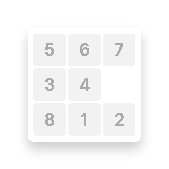
\includegraphics[keepaspectratio=true,width=5cm]{./inc/media/example_1.pdf}
\end{figure}
\paragraph{}{Sur le taquin ci-dessus, on a pour $\varepsilon{_E}(5)$:}
\begin{itemize}
\item $x{_{\textrm{\scriptsize{\li{Etat initial}}}}5 = 1}$ \hspace{2cm} $x{_{\textrm{\scriptsize{\li{Etat Final}}}}5 = 2}$
\item $y{_{\textrm{\scriptsize{\li{Etat initial}}}}5 = 1}$ \hspace{2cm} $y{_{\textrm{\scriptsize{\li{Etat Final}}}}5 = 2}$
\end{itemize}
\paragraph{}{Donc $\varepsilon{_E}(5)=2$}
\paragraph{}{Les cœfficients de normalisation correspondant sont pour une heuristique $i$:}
\begin{itemize}
\item $\rho{_{i=1}} = \rho{_{i=3}} = \rho{_{i=5}} = 4$
\item $\rho{_{i=2}} = \rho{_{i=4}} = \rho{_{i=6}} = 1$
\end{itemize}
\paragraph{}{Compte tenu du choix effectué sur la définition d’un état pour un taquin de largeur 3:}
\paragraph{A l’état initial:}
\begin{itemize}
\item Environnement:
\begin{itemize}
\item [{\ttfamily\bfseries sizes} =] {\ttfamily [3, 9]}
\item [{\ttfamily\bfseries choices} =] {\ttfamily [1, 2, 3, 4, 5, 6]}
\item [{\ttfamily\bfseries weightings} =] {\color{gray}{\em Une liste des jeux de pondérations choisis}}
\item [{\ttfamily\bfseries moves} =] {\ttfamily [Taquin Initial]}
\item [{\ttfamily\bfseries end} =] {\ttfamily []}
\end{itemize}
\item Taquin Initial:
\begin{itemize}
\item [{\ttfamily\bfseries environment} =] {\color{gray}{\em L'environnement ci-dessus}}
\item [{\ttfamily\bfseries previous} =] {\ttfamily None}
\item [{\ttfamily\bfseries sequence} =] {\ttfamily [4, 6, 2, 1, 3, 5, 0, 7, 8]} {\color{gray}{\em Une liste générée aléatoirement et valide}}
\item [{\ttfamily\bfseries inv} =] {\ttfamily 8}
\item [{\ttfamily\bfseries dis} =] {\ttfamily 8}
\item [{\ttfamily\bfseries man} =] {\ttfamily 10}
\item [{\ttfamily\bfseries path} =] {\ttfamily ""}
\item [{\ttfamily\bfseries moves} =] {\ttfamily ["L", "D"]}
\item [{\ttfamily\bfseries h} =] {\ttfamily 142}
\item [{\ttfamily\bfseries g} =] {\ttfamily 0}
\item [{\ttfamily\bfseries f} =] {\ttfamily 142}
\end{itemize}
\end{itemize}
\paragraph{A l’état final:}
\begin{itemize}
\item Taquin Final:
\begin{itemize}
\item [{\ttfamily\bfseries environment} =] {\color{gray}{\em L'environnement est toujours le même, seul l'état final est ajouté à la liste \ttfamily end}}
\item [{\ttfamily\bfseries previous} =] {\color{gray}{\em L'avant-dernier état}}
\item [{\ttfamily\bfseries sequence} =] {\ttfamily [1, 2, 3, 4, 5, 6, 7, 8, 0]}
\item [{\ttfamily\bfseries inv} =] {\ttfamily 0}
\item [{\ttfamily\bfseries dis} =] {\ttfamily 0}
\item [{\ttfamily\bfseries man} =] {\ttfamily 0}
\item [{\ttfamily\bfseries path} =] {\color{gray}{\em Le chemin minimal depuis l'état initial jusqu'à cet état}}
\item [{\ttfamily\bfseries moves} =] {\ttfamily ["R"]}
\item [{\ttfamily\bfseries h} =] {\ttfamily 0}
\item [{\ttfamily\bfseries g} =] {\color{gray}{\em La longueur du chemin minimal}}
\item [{\ttfamily\bfseries f} =] {\ttfamily g}
\end{itemize}
\end{itemize}
\subsection{Définition d’une action}
\paragraph{}{Une fois les états définis, il faut désormais s’intéresser aux actions. Une action dans ce problème est le déplacement d’une tuile, qui consiste en l'inversion de sa position avec celle du vide.}
\paragraph{}{Seule les tuiles qui jouxtent le vide sont candidates à ces déplacements et une tuiles qui vient d'être déplacée ne revient pas au coup d'après à sa position précédente pour éviter la possibilité de créer un cycle et ainsi accélerer le parcours des états. Ainsi on peut en tirer les conclusions suivantes:}
\begin{itemize}
\item Si la tuile vide se trouve à l'interieur du taquin à l'état initial, il y 4 coups possibles.
\item Si la tuile vide se trouve sur un bord du taquin (mais pas dans un coin) du taquin à l'état initial, il y 3 coups possibles.
\item Si la tuile vide se trouve dans un coin du taquin à l'état initial, il y 2 coups possibles.
\item En revanche, si l'état actuel n'est pas l'état initial, il faut retirer 1 coup à chacunes des valeurs précédentes.
\end{itemize}
\subsection{Définition de l'agent}
\paragraph{}{Il s'agit ici d'agents à réflèxes simples: les agents agissent en tenant compte du dernier percept uniquement. Nous allons donc utiliser de règles de type $\textrm{action} \Longrightarrow \textrm{condition}$}.
\subsection{Choix de l’algorithme}
\paragraph{}{Après avoir défini les états et les actions, nous nous intéressons à la stratégie utilisée par l’algorithme de recherche \textbf{A*} dans le but de trouver une séquence d’actions permettant d’atteindre l’état du but à partir de l’état initial.}
\paragraph{}{La stratégie adoptée par l’algorithme consiste en la construction d'un arbre de recherche et d’y rechercher la solution. Dans ce sens, \textbf{A*} va utiliser une fonction d'évaluation basée sur des heuristiques sur chaque nœud de l'arbre afin d’estimer le meilleur chemin à emprunter et d'en visiter les nœuds enfants, triés grâce à cette fonction d'évaluation.}
\paragraph{}{Le principe repose sur le fait qu'à chaque itération, on tente de se rapprocher de la destination, c’est pourquoi on privilégie les états directement les plus proches de la destination en mettant de côté tous les autres.}
\paragraph{}{Tous les états ne permettant pas de se rapprocher de la destination sont éloignés et placés plus loin dans la file d'éxécution. Les états parcourus sont placés dans une liste des états explorés de manière à vérifier que le chemin actuellement emprunté est plus performant que celui stocké dans la liste.}
\paragraph{}{Si cela s'avérait être le contraire, alors l'exploration actuelle s'arreterait pour passer à l'exploration d'un autre chemin. Ainsi, on est sûr d'emprunter un chemin minimal pour les heuristiques choisies et d'éviter d'explorer à nouveau un même nœud mais de coût plus élevé. C'est l'association de ces différents principes qui assure la complétude de l'algorithme.}
\subsection{Implémentation de \textbf{A*}}
\paragraph{}{Le problème majeur de \textbf{A*} est sa complexité exponentielle en espace mémoire. Tous les états créés sont conservés, ce qui peut selon les dimensions et l'état initial du taquin, rapidement saturer la mémoire de l'ordinateur, même avec les grandes capacités de mémoire actuelles.}
\paragraph{}{Par conséquent, nous nous sommes, lors de la réalisation de notre programme, chercher à réduire le nombre d’états et à établir la meilleure gestion possible de ces derniers. En ce sens, nous avons pensé judicieux d'appliquer quelques optimisations:}

%\paragraph{Améliorer l'estimation de la distance de Manhattan}{en tenant compte des conflits linéaires. L'idée est la suivante: si deux tuiles se situent sur la même ligne (respectivement même colonne), et si leurs positions sont inversées par rapport à celles souhaitées, alors l'une d'elle devra nécessairement quitter temporairement cette ligne (respectivement colonne).}
%\paragraph{}{La distance de Manhattan ne prend pas cela en compte, et on peut donc lui ajouter 2 sans risque de surestimer la distance réelle. Dans certaines positions, il existe plusieurs conflits de la sorte, et on peut donc ainsi obtenir une estimation de distance nettement plus précise que la distance de Manhattan.}
%\paragraph{}{Explorer un sommet coûte alors plus cher en temps, puisque le calcul de distance devient plus complexe. En contrepartie, le nombre de sommets à explorer diminue de façon importante, ce qui permet des gains importants en pratique."""}
\paragraph{Utiliser un dictionnaire ordonné afin de gérer la frontière}{En effet, la frontière peut comporter énormément d'états. C'est pour cela qu'il convient de trier ces états afin d'en permettre une meilleure gestion. Un dictionnaire ordonné en fonction d'une clef (la fonction d'évaluation f dans le cas présent) nous a paru le plus adapté. Cela nous permet d'éviter de parcourir la liste des états dans le but d'expanser celui possédant le f le plus petit. Grâce à cette structure, nous expansons uniquement l'état présent en premier dans le dictionnaire.}
\paragraph{Utiliser un dictionnaire pour les états explorés}{Afin de réduire le temps de traitement et diminuer les expansions, il parait logique de supprimer les états redondants et par conséquent inutiles. Ce que nous désignons par états redondants, sont en fait les états caractérisés par une séquence similaire mais un f différent. Ici, l'état qui va nous intéresser pour une même séquence est l'état possédant un f le plus petit possible.}
\paragraph{}{C'est pourquoi notre dictionnaire va ordonner les états en fonction de la séquence (transformée en chaîne de caractères). Après la création des nœuds, nous vérifions que leur séquence n'est pas similaire à celle d'un état présent dans les états explorés. Si c'est le cas : nous regardons le f. Si le f de l'enfant est supérieur à celui de l'état exploré, nous supprimons l'enfant.  Sinon, nous supprimons l'état présent dans les états explorés.}
\paragraph{}{Dans cette optique, notre dictionnaire va prendre en clef la séquence (transformée en chaîne de caractères). De même, lorsque nous expansons un état, nous l'ajoutons dans la liste des états explorés. Cette structure de donnée nous permet en outre d'optimiser le temps de recherche d'un état exploré.}



\chapter{Etude Expérimentale}
\paragraph{}{Dans cette première partie nous allons nous intéresser aux performances de l'algorithme sur des taquins 3*3. Pour cela nous exécuterons le programme sur les taquins suivants (solubles et générés aléatoirement par une fonction de notre programme): }
\begin{itemize}
\item {\ttfamily\lbrack3, 4, 0, 7, 2, 1, 8, 6, 5\rbrack}
\item {\ttfamily\lbrack5, 4, 3, 0, 7, 1, 2, 6, 8\rbrack}
\item {\ttfamily\lbrack8, 4, 5, 7, 0, 6, 3, 1, 2\rbrack}
\item {\ttfamily\lbrack0, 3, 8, 4, 6, 1, 7, 5, 2\rbrack}
\item {\ttfamily\lbrack6, 7, 5, 4, 8, 2, 0, 3, 1\rbrack}
\item {\ttfamily\lbrack6, 2, 5, 3, 4, 7, 1, 0, 8\rbrack}
\item {\ttfamily\lbrack3, 6, 5, 0, 1, 4, 8, 2, 7\rbrack}
\item {\ttfamily\lbrack3, 0, 6, 1, 8, 2, 5, 7, 4\rbrack}
\item {\ttfamily\lbrack2, 5, 7, 0, 1, 6, 8, 3, 4\rbrack}
\item {\ttfamily\lbrack0, 2, 8, 1, 4, 5, 6, 3, 7\rbrack}
\end{itemize}

\paragraph{}{A partir de ces derniers, nous collecterons des informations relatives au temps d'exécution du programme, le nombre d'états créés, l'écart à la solution optimale ainsi que le taux d'optimalité (nombre de fois moyens où la solution renvoyée est minimale) le tout en faisant varier les heuristiques.}

\paragraph{Comparaison des heuristiques individuellement}{Dans un premier temps, nous allons nous attacher à comparer les différentes heuristiques utilisées dans le but de résoudre ce problème.}
\paragraph{}{En ce sens, nous avons éxécuté 10 fois le programme en utilisant chaque heuristique afin de collecter des informations relatives au temps d'execution du programme, le nombre d'états créés, et l'optimalité de la solution:}
{\scriptsize\addfontfeatures{Numbers=Tabular}
\renewcommand{\arraystretch}{1.3}
\vspace*{.5cm}
\begin{figure}[h!]
\centering
\begin{tabular}{| c | c | c | c | c |} \hline
\textbf{ } & \textbf{Temps} & \textbf{Etats créés} & \textbf{Ecart à la Solution} & \textbf{Optimalité} \\ \hline
\textbf{H.1} & 26ms & 624 & 5,2 états & $\mathsf{\tfrac{1}{5}}$ \\ \hline
\textbf{H.2} & 18ms & 450 & 9,2 états & $\mathsf{\tfrac{1}{5}}$ \\ \hline
\textbf{H.3} & 49ms & 1524 & 0,6 états & $\mathsf{\tfrac{2}{3}}$ \\ \hline
\textbf{H.4} & 14ms & 411 & 8,8 états & $\mathsf{\tfrac{1}{5}}$ \\ \hline
\textbf{H.5} & 43ms & 1342 & 0,6 états & $\mathsf{\tfrac{2}{3}}$ \\ \hline
\textbf{H.6} & 87ms & 2831 & 0 états & 1 \\ \hline
\textbf{Désordre} & 1,2s & 36089 & 0 états & 1 \\ \hline
\end{tabular}
\end{figure}
\vspace*{.5cm}
}

% \textbf{H1} & 0,026284623 & 623,7 & 5,2 & $\frac{1}{5}$ \\ \hline
% \textbf{H2} & 0,017823386 & 450,3 & 9,2 & $\frac{1}{5}$   \\ \hline
% \textbf{H3}& 0,049105382 & 1524 & 0,6 & $\frac{2}{3}$ \\ \hline
% \textbf{H4} & 0,014410663 & 410,7 & 8,8 & $\frac{1}{5}$ \\ \hline
% \textbf{H5} & 0,042847085 & 1341,7 & 0,6 & $\frac{2}{3}$  \\ \hline
% \textbf{H6} & 0,087112284 & 2830,6 & 0 & 1  \\ \hline
% \textbf{Taux de désordre} & 1,199918461 & 36088,5 & 0& 1 \\ \hline
% ${\mathsf{\tfrac{1}{5}}}$

\paragraph{}{Nous remarquons donc que H.4 présente le temps d'exécution moyen et le nombre d'états créés moyen les plus faibles, cependant elle ne renvoie un résultat optimal qu'une exécution sur 5.}

\paragraph{}{Au contraire, les heuristiques H.6 et Désordre permettent l'obtention d'un résultat optimal mais leurs temps d'exécution se classent parmi les plus élevés.}

\paragraph{}{Cette étude soulève donc une question importante : doit-on privilégier la rapidité d'un programme au détriment de son optimalité ou au contraire favoriser un résultat minimal?}

\paragraph{}{En outre, nous pouvons remarquer que lorsque le coefficient de normalisation vaut 1, le temps moyen d'exécution ainsi que le nombre moyen d'états créés est plus faible que pour un coefficient de normalisation valant 4. L'algorithme sur-estime le chemin lorsque le coefficient de normalisation n'est pas appliqué et retourne donc rapidement un chemin de plus mauvaise qualité, fait décrit par l'écart moyen à la solution plus élevé sur les heuristiques H.1, H.2 et H.4.}

\paragraph{Comparaison de l'association d'heuristiques}{Nous allons maintenant nous pencher sur l'association de plusieurs heuristiques afin de résoudre le problème.}

{\scriptsize\addfontfeatures{Numbers=Tabular}
\renewcommand{\arraystretch}{1.3}
\vspace*{.5cm}
\begin{figure}[h!]
\centering
\begin{tabular}{| c | c | c | c | c |} \hline
\textbf{ } & \textbf{Temps} & \textbf{Etats créés} & \textbf{Ecart à la Solution} & \textbf{Optimalité} \\ \hline
\textbf{H.1 ⟶ H.6} & 78ms & 748 & 23 états & $\mathsf{\tfrac{1}{10}}$ \\ \hline
\textbf{H.6 + Désordre} & 75ms & 1753 & 0,6 états & $\mathsf{\tfrac{7}{10}}$ \\ \hline
\textbf{H.5 + Désordre}& 43ms & 913 & 1,8 états & $\mathsf{\tfrac{1}{2}}$ \\ \hline
\textbf{H.2 + H.4} & 33ms & 657 & 12,4 états &$\mathsf{\tfrac{1}{5}}$ \\ \hline
\end{tabular}
\end{figure}
\vspace*{0,5cm}
}

%\textbf{ } & \textbf{Temps} & \textbf{Etats créés} & \textbf{Ecart à la Solution} & \textbf{Optimalité} \\ \hline
%\textbf{H1 H2 H3 H4 H5 H6} & 0,077811193 & 747,6 & 23 & ${\mathsf\tfrac{1}{10}}$ \\ \hline
%\textbf{H6 Taux de désordre} & 0,074782300 & 1753 & 0,6 & ${\mathsf\tfrac{7}{10}}$   \\ \hline
%\textbf{H5 Taux de désordre}& 0,043249559 & 913,2 & 1,8 & ${\mathsf\tfrac{1}{2}}$ \\ \hline
%\textbf{H2/H4}&0,032602048&656,8&12,4&$\frac{1}{5}$\\ \hline

\paragraph{}{Tout d'abord, nous pouvons noter que lors de l'utilisation simultanée de toutes les heuristiques, l'écart moyen à la solution est très élevé et le taux d'optimalité extrêmement faible. De plus, le temps d'exécution moyen se classe parmi les plus élevés.}
\paragraph{}{Néanmoins, deux heuristiques nous semblaient intéressantes à combiner: la distance de Mahnattan avec une pondération de 1 ainsi que le taux de désordre. Il s'avère en effet que ces deux heuristiques optimales 10 fois sur 10 tentatives et possédant un temps et un nombre d'états créés moyens très élevés séparément se révèlent être des alliées redoutables lorsqu'elles travaillent de pair. Effectivement, l'écart moyen de leur concours à la solution optimal est minime : 0,6 états et leur taux d'optimalité acceptable: $\mathsf{\tfrac{7}{10}}$.}

\paragraph{}{De même, les heuristiques H.5 et le taux de désordre combinés proposent de bonne performances au niveau du temps d'exécution et du nombre d'états moyen créés. Cependant l'écart moyen à la solution optimale est 3 fois supérieur à celui de H.6 et taux de désordre combinés. Le taux d'optimalité est par ailleurs faible: 1 fois sur 2.}

\paragraph{}{Pour finir, nous avons tenté de combiner H.2 ainsi que H.4, les deux heuristiques qui dissociées présentent les temps moyen ainsi que le nombre moyen d'états créés le plus faible. Toutefois nous pouvons constater que leur concours présente des performances inférieures et un taux d'optimalité équivalent.}
\chapter{Extensions}
\section{TAQUINS 4*4}
\paragraph{}{Intéressons nous maintenant à la résolution de taquins 4*4 par notre algorithme. Pour cela nous allons collecter des données relatives au temps moyen d'exécution, le nombre d'états moyens créés et le nombre de coups moyen pour parvenir à résoudre le problème.}
\paragraph{}{De même que lors de la partie précédente, nous collecterons ces données à partir de taquins solubles générés aléatoirement. Ces taquins sont les suivants:}
\begin{itemize}
\item {\ttfamily\lbrack  0,  7,  3, 12, 14, 13,  5,  9, 10,  6, 11, 15,  1,  2,  8,  4\rbrack}
\item {\ttfamily\lbrack  5, 14,  3,  9,  2,  0, 10,  1,  4, 15, 11,  6, 13,  7,  8, 12\rbrack}
\item {\ttfamily\lbrack  1, 12,  8,  7,  2, 10,  3,  9,  0,  6,  5, 14,  4, 11, 13, 15\rbrack}
\item {\ttfamily\lbrack 13, 11, 12,  8, 15,  1,  0,  3,  7, 14,  9,  4,  5,  2,  6, 10\rbrack}
\item {\ttfamily\lbrack  9,  2,  4, 14,  3, 11,  8, 15, 12,  5,  1,  7, 13,  0,  6, 10\rbrack}
\item {\ttfamily\lbrack 14,  7,  8, 11, 10,  6,  1, 12, 15,  0,  5,  3,  9,  2, 13,  4\rbrack}
\item {\ttfamily\lbrack  4,  7,  5,  0, 13, 11,  1, 12, 15, 10,  9,  3,  8,  2, 14,  6\rbrack}
\item {\ttfamily\lbrack 14, 12, 11,  6,  9, 15,  3,  1,  2,  5, 10, 13,  8,  4,  0,  7\rbrack}
\item {\ttfamily\lbrack  2,  3, 14,  8,  0,  9, 13,  6, 10,  4,  7,  1, 15, 12,  5, 11\rbrack}
\item {\ttfamily\lbrack  7, 15,  2, 12,  1,  6,  5,  3, 10,  4, 11, 14, 13,  0,  8,  9\rbrack}
\end{itemize}
\paragraph{}{Cependant, pour la résolution des taquins 4*4 nous avons pris la liberté de modifier le coefficient de normalisation de H6. Ce dernier vaut désormais $\mathsf{\tfrac{1}{2}}$. Sans cette modification, H.6 sous estimait grandement le chemin et par conséquent une exécution du programme avec cette dernière pouvait prendre plus d'une heure.}
{\scriptsize\addfontfeatures{Numbers=Tabular}
\renewcommand{\arraystretch}{1.3}
\vspace*{.5cm}
\begin{figure}[h!]
\centering
\begin{tabular}{| c | c | c | c |} \hline
\textbf{ } & \textbf{Temps} & \textbf{Etats créés} & \textbf{Nombre de Coups}\\ \hline
\textbf{H.1} & 87s & 1239868 & 64 \\ \hline
\textbf{H.2} & 2s & 34478 & 120 \\ \hline
\textbf{H.3} & 7s & 124682 & 67 \\ \hline
\textbf{H.4} & 2s & 36173 & 117 \\ \hline
\textbf{H.5} & 3s & 45226 & 65\\ \hline
\textbf{H.6} & 5s & 86995 & 61 \\ \hline
\textbf{H.1 ⟶ H.6}&5s&29990&160\\ \hline
\textbf{H.6 + Désordre}&4s&50553&68\\ \hline
\end{tabular}
\end{figure}
}
% \textbf{H.1} & 86,852147675 & 1239867,5 & 64,1 \\ \hline
% \textbf{H.2} & 2,358877850 & 34478,3 & 120,3 \\ \hline
% \textbf{H.3} & 7,183158445 & 124681,6 & 67,3 \\ \hline
% \textbf{H.4} & 2,345959473 & 36172,6 & 116,9 \\ \hline
% \textbf{H.5} & 2,548957515 & 45226,2 & 65,3\\ \hline
% \textbf{H.6} & 4,902488279 & 86994,7 & 61,3 \\ \hline
% \textbf{H1/H2/H3/H4/H5/H6}&5,448457384&29989,8&159,5\\ \hline
% \textbf{H6/Taux de désordre}&4,026388192&50552,5&68,1\\ \hline

\paragraph{Utilisation des heuristiques en simultané}{Dans un premier temps, nous pouvons noter que lors de l'utilisation simultanée de toutes les heuristiques, l'algorithme sur-estime grandement le chemin et par conséquent le nombre de coups moyen est très élevé.}
\paragraph{Comparaison des heuristiques séparément}{Dans un second temps, nous constatons que pour la résolution d'un taquin 4*4, l'heuristique H.6 (avec un coefficient de normalisation modifié) paraît la plus judicieuse à utiliser. En effet, elle présente le nombre de coups moyen le plus faible et un temps moyen ainsi qu'une utilisation de l'espace mémoire raisonnable. Par opposition, l'heuristique H.1 semble être à éviter puisque son temps moyen et son espace mémoire utilisé est déraisonnable.}
\paragraph{H.6 + Désordre}{Nous remarquons également que l'association H.6 + Désordre produit un résultat convenable également. Cependant, son nombre de coups moyen étant supérieur à H.6 utilisée seule, nous ne retiendrons pas cette combinaison.}
\paragraph{Conclusion}{Nous pouvons en conclure que la meilleure heuristique pour résoudre un taquin 4*4 est H6 avec un coefficient de normalisation valant $\mathsf{\tfrac{1}{2}}$ ; dans les faits, ce dernier multiplie la valeur de la distance de Manhattan non pondérée par 2.}
\section{TAQUINS 5*5}
\paragraph{Résolution des Taquins 5*5}{Afin de résoudre de façon rapide un Taquin 5*5, nous utilisons l'algorithme IDA* et les heuristiques H6 (avec un coefficient de normalisation de $\mathsf{\tfrac{1}{3}}$) ainsi que Taux de Désordre. Sur 10 exécutions on obtient : }
\begin{itemize}
\item Un temps moyen de : 57 secondes
\item Un nombre d'états moyens créés de : 402562,8 états
\item Un nombre de coups moyens de : 232,4 coups
\end{itemize}
\section{Implémentation d'un autre algorithme de recherche}
\paragraph{L'algorithme IDA*}{Nous avons choisi d'implémenter une variante de l'algorithme \textbf{A*} : IDA*. Son fonctionnement est similaire à celui de \textbf{A*} mais avec une recherche en profondeur itérative.}
\paragraph{}{L'algorithme fonctionne comme suit: à chaque itération, on effectue une recherche en profondeur d'abord, en coupant une branche lorsque son coût total
$\mathsf{f(n) = g(n) + h(n)}$ dépasse un seuil donné. Ce seuil commence à l'estimation du coût à l'état initial et augmente à chaque itération de l'algorithme. Ainsi, le seuil utilisé pour l'itération suivante est le coût minimum de toutes les valeurs dépassant le seuil actuel.

Comme dans \textbf{A*}, l'heuristique doit avoir des propriétés particulières pour garantir l'optimalité de la solution. Nous utiliserons donc les même heuristiques que précédemment.}

\paragraph{Exemple d'exécution : }{Un exemple d'exécution de l'algorithme (en utilisant les heuristiques 6 et Taux de désordre) est le suivant : }
\begin{itemize}
\item \textbf{Taquin : } \lbrack3, 5, 2, 4, 1, 7, 0, 6, 8\rbrack
\item \textbf{Temps : }IDA* :  0.184770107 secondes / \textbf{A*} : 0.063782215 secondes
\item \textbf{Nombre d'états créés :} IDA* : 4426 / \textbf{A*} : 1206
\item \textbf{Nombre de coups réalisés : } IDA* : 20 / \textbf{A*} : 20
\end{itemize}

\section{Création de nouvelles heuristiques}
\paragraph{}{Afin de permettre une meilleure résolution des taquins (en temps, espace et optimalité), nous avons créé de nouvelles heuristiques : }
\paragraph{Le taux de désordre}{Cette heuristique calcule le nombre de tuiles mal placées dans le taquin. Comme vu dans les expériences précédentes, cette heuristique combinée à d'autres (H.6 par exemple) s'avère très utile et performante.}
\paragraph{Une heuristique qui attribue les poids de manière aléatoire}{un algorithme génère des paires de nombres allant de 1 au nombre de tuiles totales dans le taquin. Par exemple pour un taquin 3*3, nous aurons une paire de 1, une paire de 2, 1 paire de 3, une paire de 4. Puis nous mélangeons ces chiffres de façon aléatoire afin de générer les poids. Un exemple de mélange obtenu est le suivant : \lbrack2, 1, 2, 4, 1, 4, 3, 3\rbrack. Nous avions créé cette heuristique à but expérimental, mais cette dernière présente de bonnes performances sur les taquins 3*3, 4*4, et combinée à une autre heuristique (H.6 par exemple) elle peut également résoudre des taquins 5*5.}
\section{Interface graphique}
\paragraph{}{Dans l'intention de mettre en valeur notre programme, nous avons jugé opportun de réaliser une interface graphique en utilisant PyQt5. Cette interface nous permet de générer aléatoirement un Taquin et de le résoudre. Pour cela, on doit renseigner : }
\begin{itemize}
\item une largeur de Taquin parmi : 3, 4, 5
\item un mode : le mode 'Manuel' ou le mode 'Pilot'.
\begin{enumerate}
\item Le mode 'Manuel' permet de générer un taquin jouable.
\item Le mode 'Pilot' permet de générer un taquin avec des indications du "prochain meilleur coup". En effet, après chaque déplacement de tuiles, il colore en bleu la tuile correspondant au  mouvement suivant à effectuer. Ce mode n'est disponible que pour les taquins 3*3.
\end{enumerate}
\item les heuristiques à utiliser
\item un algorithme de recherche : IDA* ou \textbf{A*}
\end{itemize}
\paragraph{}{A partir de ces renseignements, le programme va générer un Taquin aléatoire sur lequel nous pourrons jouer et demander la solution à n'importe quel moment et autant de fois que désiré.}
\paragraph{}{Une fois le Taquin résolu, une fenêtre s'ouvre récapitulant les performances du joueur : le nombre de mouvements qu'il a effectué, le temps qu'il a mis pour résoudre le Taquin et la séquence de mouvements effectués. S'il s'agit d'un Taquin 3*3, il affichera le chemin minimal calculé par l'algorithme à partir du Taquin initial ainsi que le nombre de coups minimal pour résoudre ce dernier.}
\section{Interface Web}{Des le départ, une version web du programme a été mise en place pour mettre en forme plus facilement et plus rapidement une maquette de notre programme python. La version web étant totalement fonctionnelle, le langage JavaScript permet de meilleures performances et une plus grande liberté sur la conception de l'interface. Aussi, la version web est une réelle traduction de notre programme python mais disponible sur tout périphérique doté d'un navigateur. {\ttfamily\bfseries https://originecode.github.io/Taquin}}
\section{Conclusion globale}
\paragraph{}{En conclusion, l'algorithme \textbf{A*} parvient toujours à trouver une solution au problème. Cependant selon les heuristiques utilisées les solutions ne sont pas toujours optimales en nombre de coups mais aussi en temps et en espace. On remarque par ailleurs que bien souvent pour atteindre une solution optimale le temps de calcul est très long.}

\begin{figure}[!h]
\vspace{1cm}
\centering

\includegraphics[keepaspectratio=true,width=3cm]{./qrcode.pdf}
\caption{Vous trouverez ici les fichiers du projet et du rapport.}
\end{figure}

\end{document}